\section{Analysis strategy}\label{chap5:analysis_strategy}

\subsection{Event reconstruction}

Regarding electrons, muons, jets and \MET definition and reconstruction, the standard CMS recommendations described in Chapter~\ref{chap2} are used. The specific selections used in this analysis are briefly summarized below.

Muons are identified according to the definition described in Sec.~\ref{sec:muID}, with some specific modifications regarding the impact parameters of the tracks with respect to the primary vertex. In particular the requirements are lowered to $d_{xy}<0.01$\,cm and $d_z < 0.1$\,cm with respect to the \emph{tight muon selection} illustrated in Table~\ref{tab:tightmuon}.

%\begin{itemize}
%\item identified by the standard medium muon selection described in Sec.~\ref{sec:Objects}; \textcolor{red}{Not yet defined :)}
%\item $\pt> 10$\GeV;
%\item $|\eta < 2.4|$;
%\item $|d_{xy}| < 0.01$\,cm for $\pt < 20$\GeV and $|d_{xy}| < 0.02$\,cm for $\pt > 20$\GeV, $d_{xy}$ being the transverse impact parameter with respect to the primary vertex;
%\item $|d_{z}| < 0.1$\,cm, where $d_z$ is the longitudinal distance of the muon track in the tracker extrapolated along the beam direction.
%\end{itemize}

The PF relative isolation described in Eq.\eqref{eq:isomu} is used for muon isolation, corresponding to a requirement on the isolation variable of $I^{rel}_{\Delta\beta} < 0.15$. In addition a tracker relative isolation is also applied.

The tight working point described by the requirements in Table~\ref{tab:tightele} is used for the electron identification. Some additional requirements to make the selection ``trigger-safe'' are included. This is done because the electron triggers already include some identification and isolation requirements that are based on the raw detector information, while the offline selections make use of particle flow requirements. The ``trigger-safe'' selections are defined to make the offline identification and isolation requirements tighter with respect to the online triggers.

The simulated events are corrected for the lepton trigger, identification and isolation efficiencies measured in data using the same techniques described in Sec.~\ref{sec:Selections}.

Jets are obtained clustering the particle flow objects using the anti-$k_t$ algorithm with a distance parameter of 0.4. The CHS pile-up mitigation technique is used and the jet energy corrections are applied, as described in Sec.~\ref{sec:jec}. 
To reject jets arising from calorimeter or readout electronics noise, the loose working point for PF jet identification is used (see Sec.~\ref{sec:jetID}). The jet counting used in the event selection is based on jets with $\pt>30$\GeV.

\subsection{B tagging performance}

The b tagging algorithm is chosen comparing the performance of different algorithms on simulated \hwwllnn signal produced via the ggH mechanism and \ttbar background.

The b veto efficiency, $\epsilon_\text{b veto}$, is computed separately for the two samples and for various b tagging algorithms. To compare the b tagging performance, $\epsilon_\text{b veto}$ is computed for different working points, i.e. different selections on the specific b tagging discriminator, and the results are reported in the form of a ROC curve. In general, ROC curves are built reporting the signal efficiency on the $x$ axis and the background rejection on the $y$ axis. In this case the $x$ axis shows the b-jets veto efficiency for signal ($\epsilon_\text{b veto}^\text{ggH}$) and the $y$ axis the \ttbar background rejection ($1-\epsilon_\text{b veto}^{\ttbar}$). The best algorithm is the one that provides the highest background rejection for a given signal efficiency. 

The ROC curves corresponding to events with 0, 1 and $\geq 2$ jets are shown in Fig.~\ref{fig:btag}. Events considered for this study are the ones related to the typical \hww phase space. Here 0 jets means that events do not contain any jet with \pt above 30\GeV. In this category the b veto rejects the event if at least one jet with $20\GeV < \pt < 30\GeV$ is identified by the b tagging algorithm. Events containing exactly one jet with $\pt>30$\GeV are rejected if that jet is b-tagged, while events with 2 or more jets are rejected if at least one jet is b-tagged.

\begin{figure}[htb]
\centering
\subfigure[$N_\mathrm{jets} = 0$]{
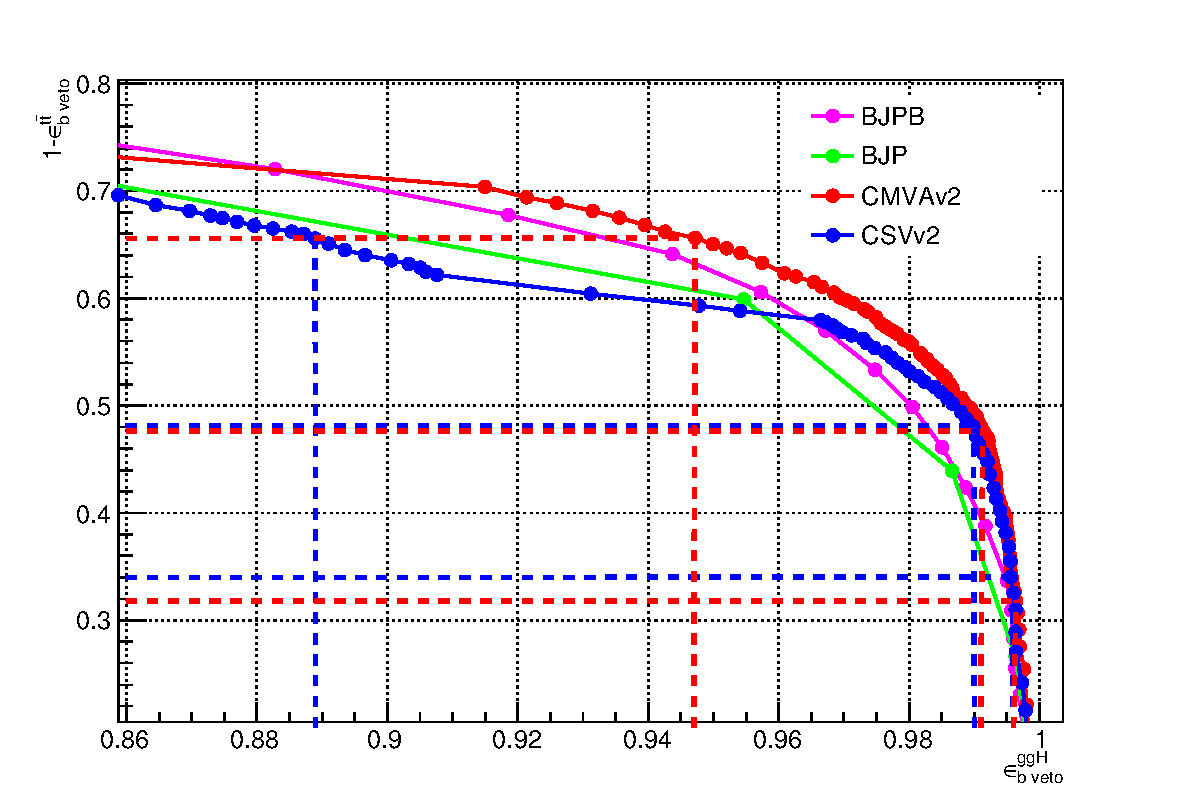
\includegraphics[width=0.45\textwidth]{images/13TeV/ROC_njet0.pdf}
}
\subfigure[$N_\mathrm{jets} = 1$]{
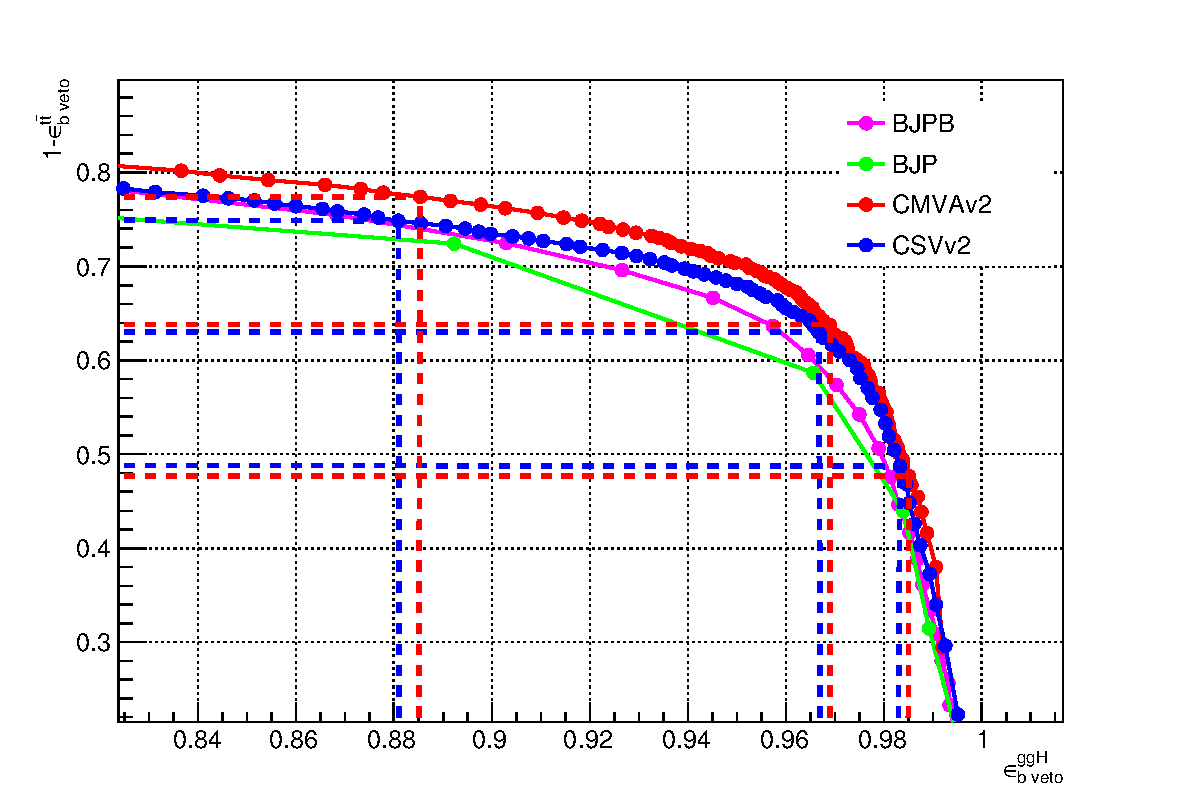
\includegraphics[width=0.45\textwidth]{images/13TeV/ROC_njet1.pdf}
}
\subfigure[$N_\mathrm{jets} \geq 2$]{
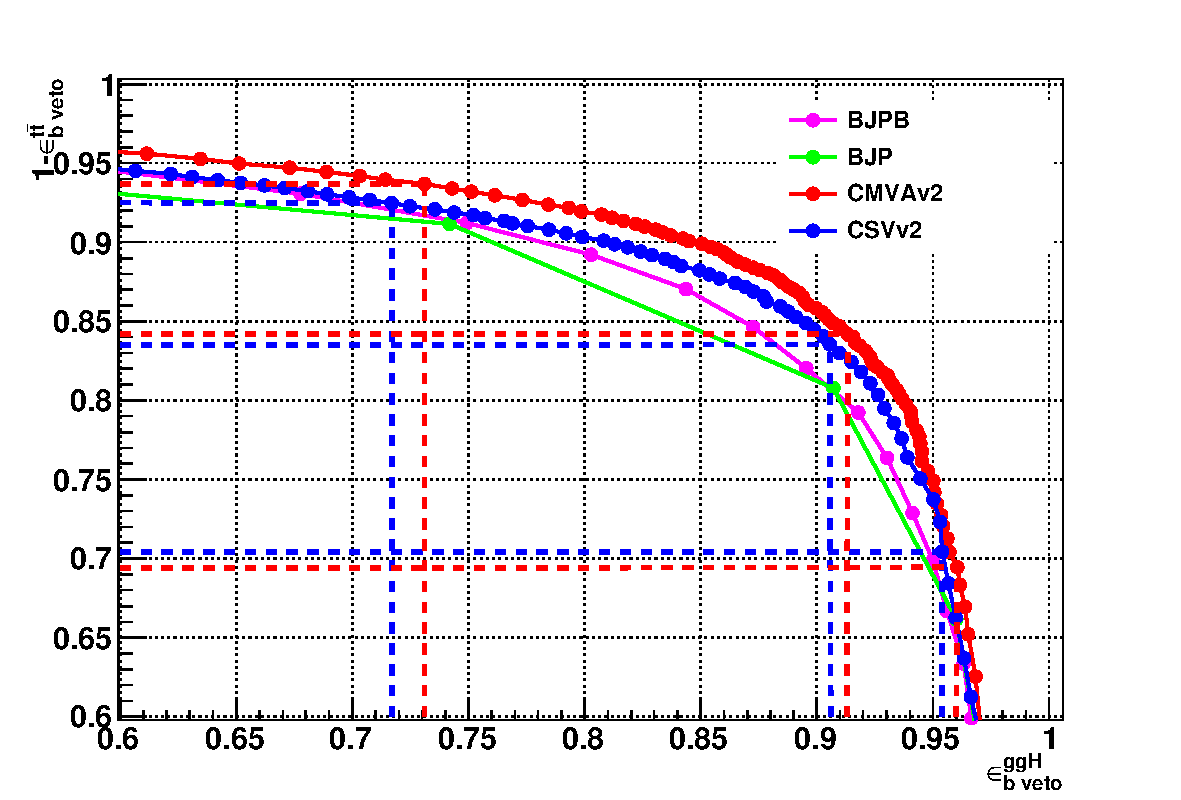
\includegraphics[width=0.45\textwidth]{images/13TeV/ROC_njetge2.pdf}
}
\caption{ROC curve for the b veto efficiency on signal and background events. The blue and red lines point out the signal efficiency and the background rejection corresponding to the three working points considered for the CSVv2 and the cMVAv2 algorithms
respectively.}\label{fig:btag}
\end{figure}

The ROC curves show that the cMVAv2 algorithm has the best performance for the analysis phase space among the algorithms taken into account. For both the CSVv2 and cMVAv2 algorithms\footnote{The CSVv2 and cMVAv2 algorithms are improved versions of the CSV and cMVA described in Sec.~\ref{sec:btag}, developed by CMS for the 13\TeV data taking period.}, three working points are defined corresponding to the mistag rates (see Sec.~\ref{sec:btag}) of 10\% (loose), 1\% (medium) and 0.1\% (tight). These mistag rates correspond roughly to $1-\epsilon_\text{b veto}^\text{ggH}$ in events with 1 jet. The distribution of the cMVAv2 discriminator associated to the leading jet for both the ggH and \ttbar samples is shown in Fig.~\ref{fig:discriminator}. The events falling on the left side of the vertical lines, which corresponds to the three working points of the cMVAv2 algorithm, are those that pass the b veto requirement.

\begin{figure}[htb]
\centering
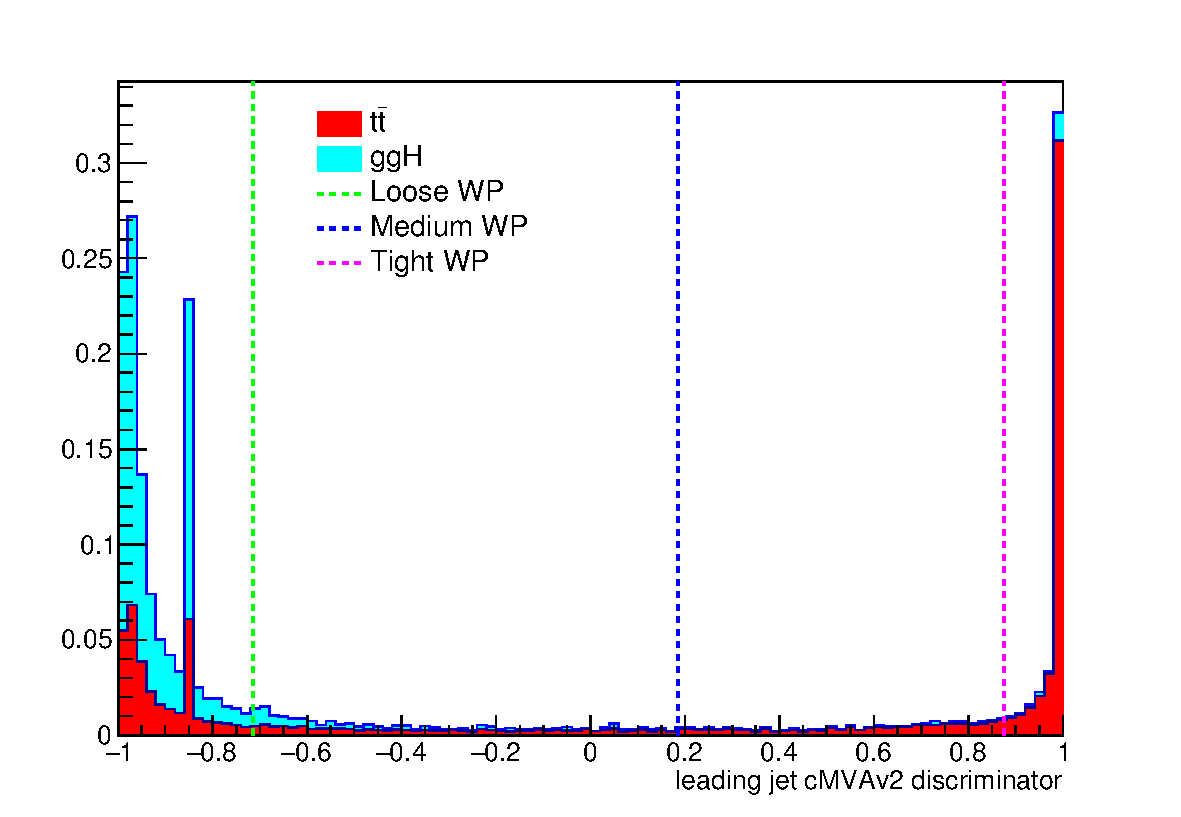
\includegraphics[width=0.6\textwidth]{images/13TeV/cmva_WP.pdf}
\caption{cMVAv2 discriminator associated to the leading jet (with $\pt > 30$\GeV) for both the ggH and the \ttbar processes. The two processes are normalized to unity and stacked. The vertical dashed lines show the discriminator value corresponding to the three working points.}\label{fig:discriminator}
\end{figure}

In order to determine the best working point for this analysis a signal significance assessment is performed, in which only statistical uncertainties are taken into account. The expected signal significance is calculated applying the event selections and using the statistical procedure described in the next sections, testing the effect of the b veto for the three working points.
The signal significance is computed for the two jet categories separately and eventually for the combination of the two. This leads to the values listed in Table~\ref{tab:significance_wp_combine} for the three working points. The loose working point is found to be the one for which the best signal significance is achieved in the combined $0+1$ jets category, and is thus chosen for the definition of the b veto requirement.

\begin{table}
\caption{Signal significance corresponding to the three working points of the cMVAv2 algorithm and for
different jet categories.\label{tab:significance_wp_combine}}
\begin{center}
\begin{tabular}{lccc}
\toprule
Jet category & Loose WP (-0.715) & Medium WP (0.185) & Tight WP (0.875) \\
\midrule
0 jets & 2.022 & 2.043 & 2.036 \\
1 jet & 1.439 & 1.404 & 1.305 \\
$0+1$ jets & 2.481 & 2.479 & 2.420 \\
\bottomrule
\end{tabular}
\end{center}
\end{table}

To correct for a possible different b tagging efficiency in data and simulation, the simulated events are reweighted using scale factors computed in bins of the jet $\eta$ and \pt.
The scale factors related to the b tagging efficiency and mistag rate, together with the corresponding uncertainties, are estimated in data and simulation adopting a Tag and Probe technique similar to the one described in Sec.~\ref{sec:ScaleFactors}.

The efficiency in simulation has to be computed for different jet flavours, i.e. b, c and light (u, d, s), using jet matching information\footnote{There are different techniques developed by the CMS Collaboration to assess the flavour of a reconstructed jet in simulation. The technique used here makes use of the flavour of the hadrons clustered into a jet.}.
The efficiencies for tagging b-, c- and light-jets estimated using simulated \ttbar events are shown in Fig.~\ref{fig:effmc} in $\eta$ and \pt bins. The uncertainties associated to the efficiencies are representative of the statistics of the simulated \ttbar sample, and are computed according to a binomial distribution.

\begin{comment}
These scale factors and the corresponding uncertainties are centrally calculated for each working point, in such a way to be employable by all the CMS analyses. The prescription to reweight the simulated events is the following. First of all one has to compute the b tagging efficiency using the MC samples, $\varepsilon_\mathrm{MC}(p_\mathrm{T}, \eta, f)$, for the chosen working point in bins of jet \pt and $\eta$. The efficiency has to be computed for different flavours $f$ of the jets, b, c and light (u,d,s), using the jet matching information\footnote{There are a couple of techniques developed by the CMS Collaboration to assess the flavour of a reconstructed jet in simulation. The technique used here makes use of the flavour of the hadrons clustered into a jet.} which is available in all the MC samples. An MC-based event weight is then calculated computing the probability $P_\mathrm{MC}$ of a given b tagging configuration to occur, e.g.:
\begin{equation}
P_\mathrm{MC}=\prod_{i~\in{}~b-tagged-jets}\varepsilon_{\mathrm{MC}_{i}}\prod_{j~\in{}~non-b-tagged-jets}(1-\varepsilon_{\mathrm{MC}_{j}})
\label{eq:btagpmc}
\end{equation}
Afterwards, a similar probability is computed using data:
\begin{equation}
P_\mathrm{DATA}=\prod_{i~\in{}~b-tagged-jets}SF_{i}\varepsilon_{\mathrm{MC}_{i}}\prod_{j~\in{}~non-b-tagged-jets}(1-SF_{j}\varepsilon_{\mathrm{MC}_{j}}) \quad ,
\label{eq:btagpdata}
\end{equation}
where $SF_{i}$ is the provided scale factor value for the relevant jet flavour, \pt and $\eta$. Products in Eqs.~\ref{eq:btagpmc} and \ref{eq:btagpdata} run over all jets. The event weight is finally given by the ration $P_\mathrm{DATA}/P_\mathrm{MC}$.

The b tagging efficiencies to be fed into Eq.~\ref{eq:btagpmc} and
Eq.~\ref{eq:btagpdata} are derived using \ttbar simulated events and applying basic leptonic
selections. These efficiencies are shown in Fig.~\ref{fig:effmc} for light
(a), c-jets (b) and b-jets (c), in bins of $\eta$ and \pt. The uncertainties associated to the efficiencies are representative of the statistics of the simulated \ttbar sample, and are computed according to a binomial distribution.
\end{comment}
\begin{figure}[!h]
\centering
\subfigure[]{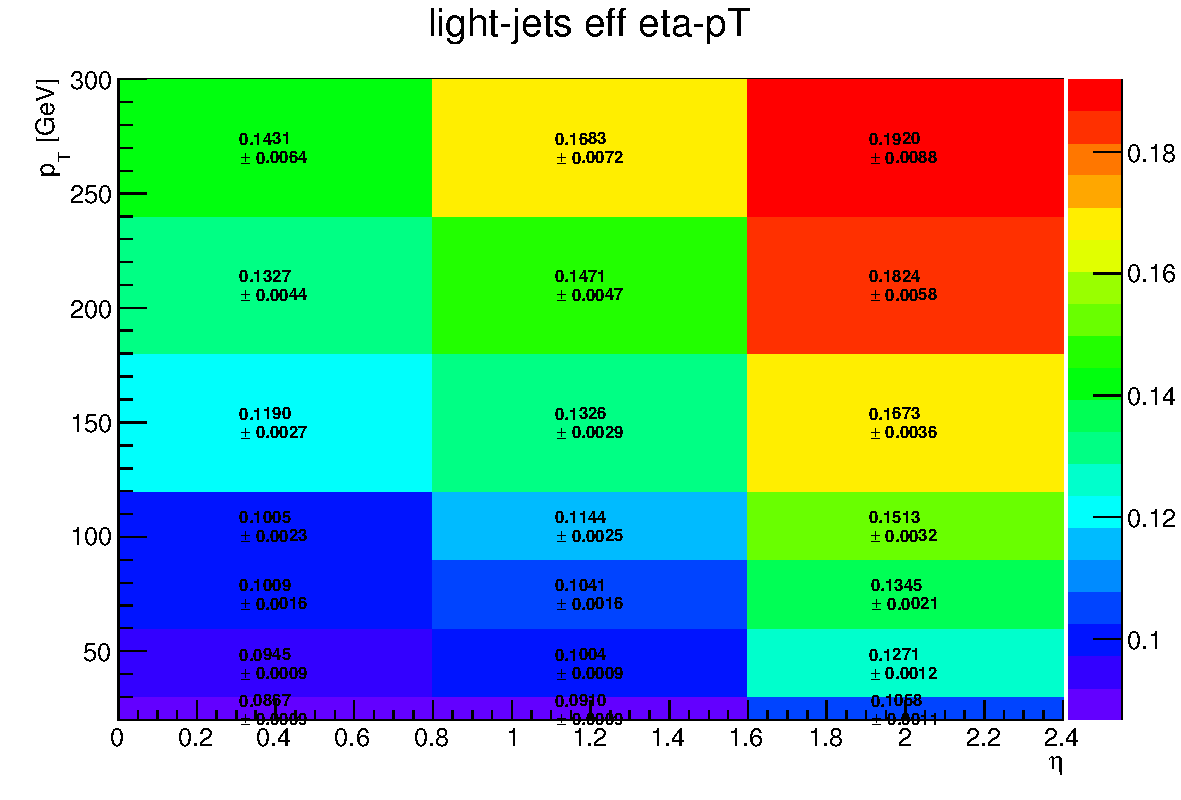
\includegraphics[width=0.4\textwidth]{images/13TeV/ljet_effmc.pdf}}
\subfigure[]{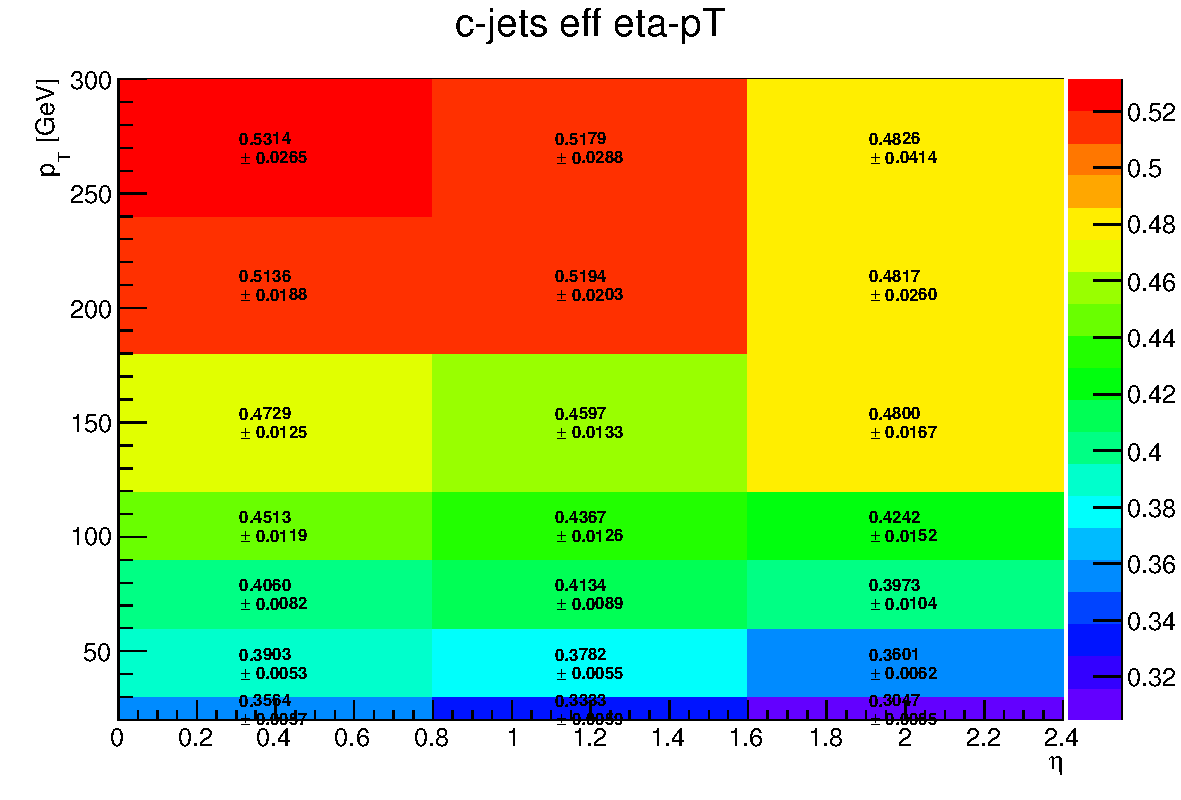
\includegraphics[width=0.4\textwidth]{images/13TeV/cjet_effmc.pdf}}\\
\subfigure[]{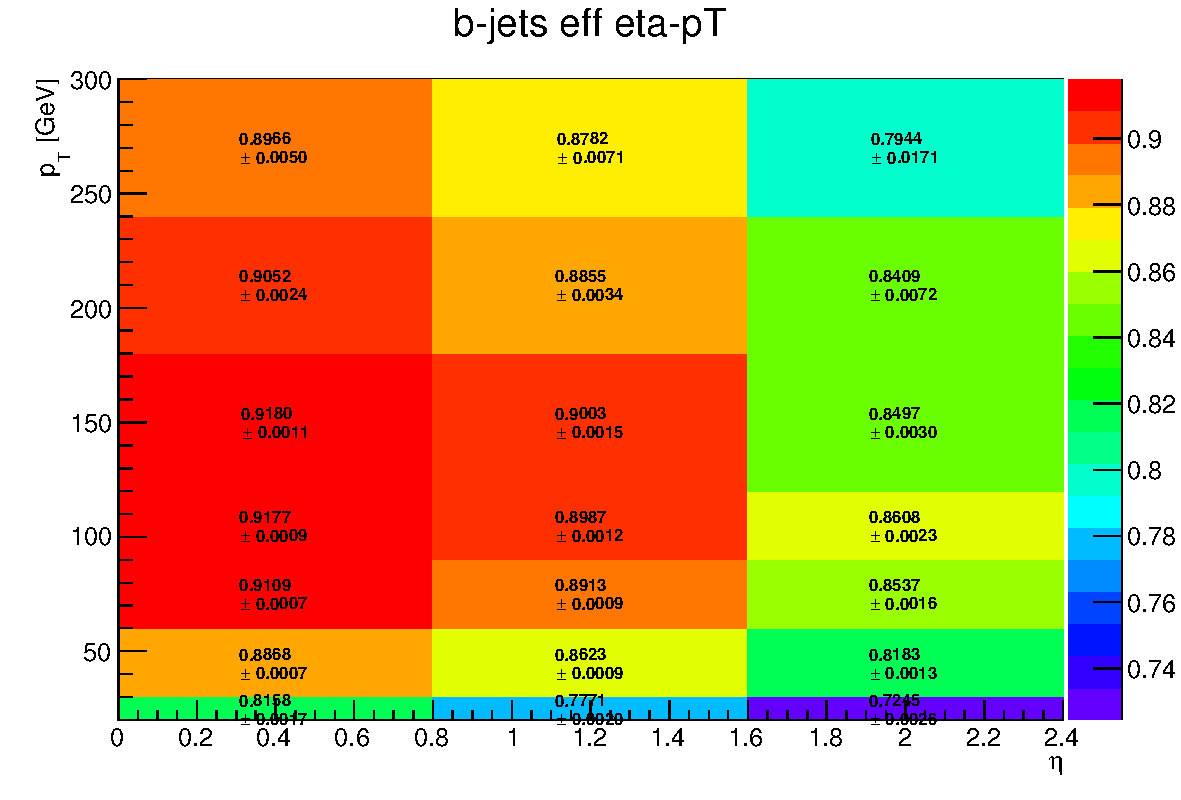
\includegraphics[width=0.4\textwidth]{images/13TeV/bjet_effmc.pdf}}
\caption{B tagging efficiencies for light jets (a), c-jets (b) and
b-jets (c), as a function of $\eta$ and \pt.\label{fig:effmc}}
\end{figure}

The effect of the event reweighting is to correct the shape of the b tagging discriminator in simulation, moving events from the b tag region (discriminator greater than $> -0.715$) to the b veto region (discriminator $ < -0.715$) and viceversa. A data/simulation comparison of the b tagging discriminator for the leading and subleading jets is performed to check the agreement after the application of the event weights. In order to evaluate the data/simulation agreement for b-jets, the data and simulation are compared to each other in a top quark enriched control region, defined by the following requirements:
\begin{itemize}
\item two leptons, an electron and a muon with opposite charge, with
leading lepton \pt greater than 20\GeV and subleading lepton \pt greater than 15\GeV;
\item no other electron or muon with \pt greater than 10\GeV;
\item \mll greater than 50\GeV;
\item at least two jets with \pt greater than 30\GeV;
\item at least one of the two leading jets with cMVAv2 b tagging score
greater than -0.715 (loose working point).
\end{itemize}
In order to evaluate the agreement for light jets, a second
control region is defined, populated by Z+light jet events, defined as follows:
\begin{itemize}
\item two electrons or two muons with opposite charge, with
leading lepton \pt greater than 20\GeV and subleading lepton \pt greater than 15\GeV;
\item no other electron or muon with \pt greater than 10\GeV;
\item \mll between 80\GeV and 110\GeV;
\item at least two jets with \pt greater than 30\GeV;
\item no jets above 20\GeV with a TCHE score above 2.1. 
\end{itemize}
Although the Z+jets sample is dominated by light flavor jets, a b-veto on an
alternative algorithm (TCHE) is applied to reduce the contamination from b-jets,
especially above the cMVAv2 cut. This helps mitigating possible discrepancies between data and simulation in the modelling of the heavy/light flavour ratio.
The comparison of the discriminator shape in data and simulation after the event reweighting is shown in Figs.~\ref{fig:bpogSF} and \ref{fig:bpogSF_Z} for the b-jets and light jets enriched control regions, respectively. The discriminator distribution is displayed in two bins and the edge represents the discriminator cut, in this case the one corresponding to the loose working point. Therefore, the entries falling in the left (right) bin correspond to events in which the leading or subleading jet fails (passes) the b tagging selection.

\begin{figure}[htb]
\centering
\subfigure[]{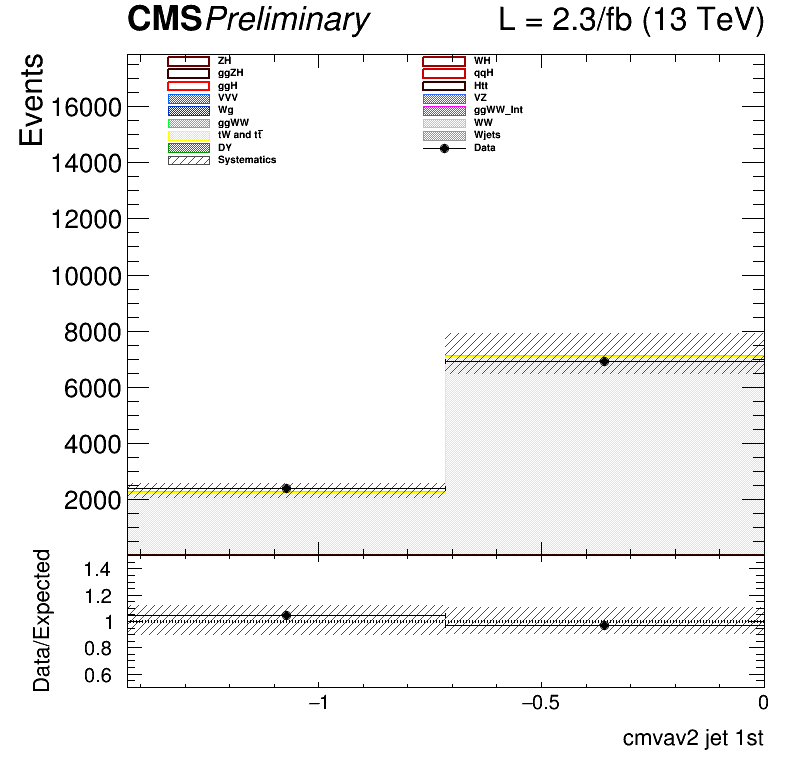
\includegraphics[width=0.4\textwidth]{images/13TeV/cratio_hww2l2v_13TeV_top_of1j_cmva_twobins_1.png}}
\subfigure[]{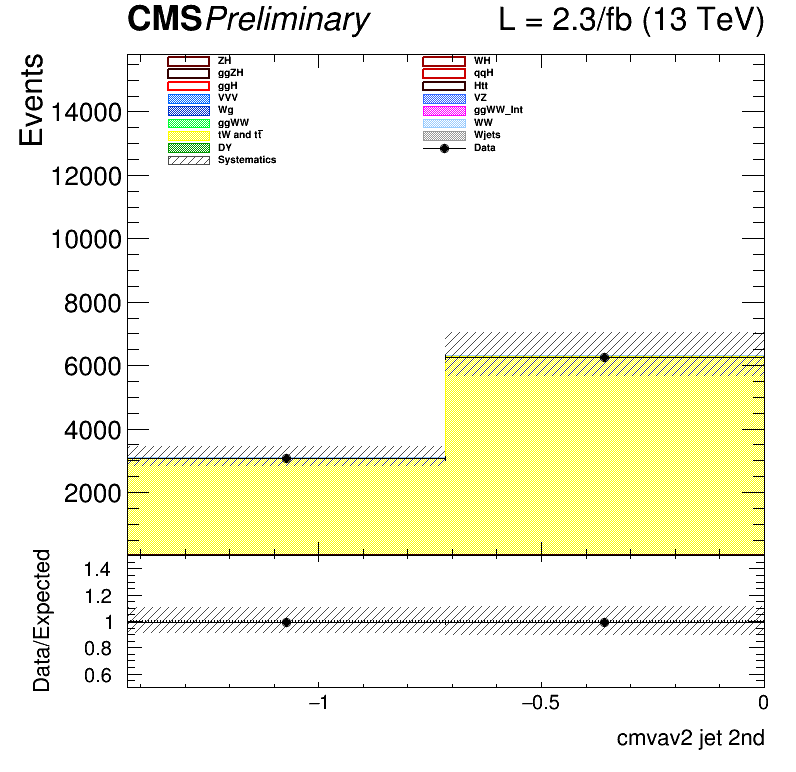
\includegraphics[width=0.4\textwidth]{images/13TeV/cratio_hww2l2v_13TeV_top_of1j_cmva_twobins_2.png}}
\caption{cMVAv2 discriminator for the leading (a) and subleading (b)
jet in the b-jets enriched control region.\label{fig:bpogSF}}
\end{figure}
\begin{figure}[htb]
\centering
\subfigure[]{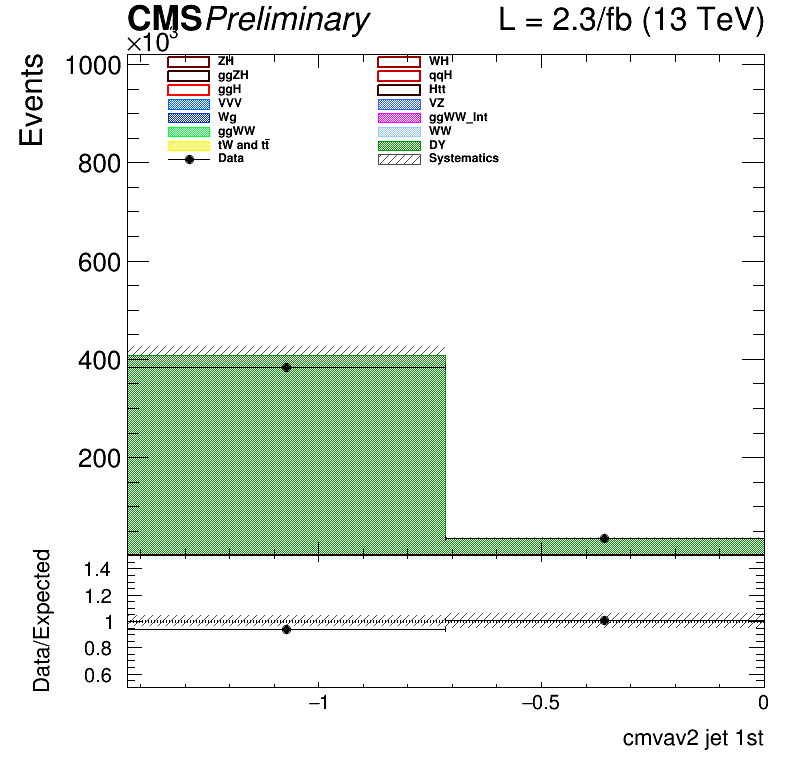
\includegraphics[width=0.4\textwidth]{images/13TeV/cratio_ZjetsCutTCHE_mumu_cmva_twobins_1.png}}
\subfigure[]{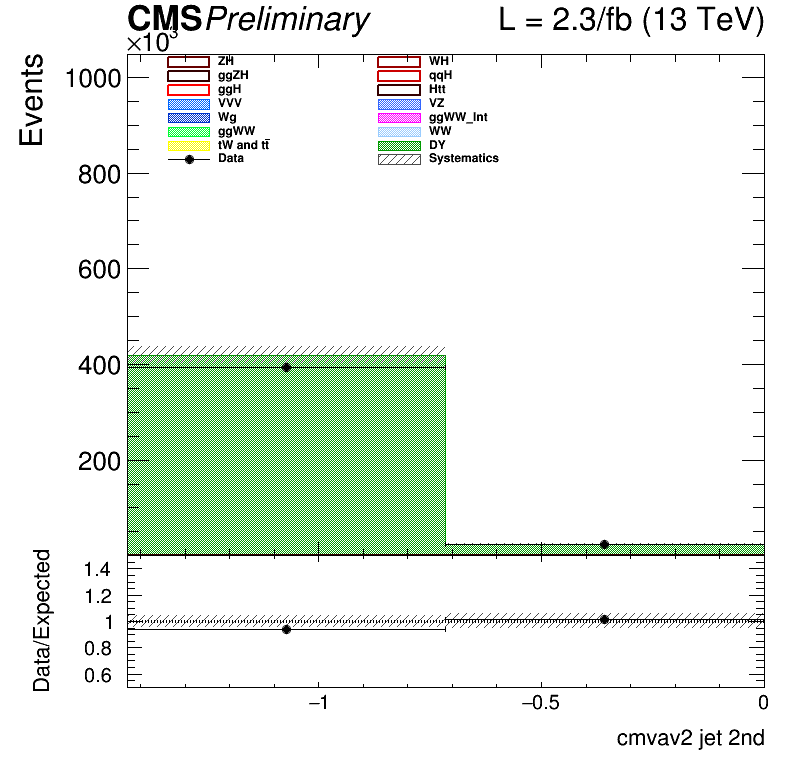
\includegraphics[width=0.4\textwidth]{images/13TeV/cratio_ZjetsCutTCHE_mumu_cmva_twobins_2.png}}
\caption{cMVAv2 discriminator for the leading (a) and subleading (b)
jet in the light jets enriched control region.\label{fig:bpogSF_Z}}
\end{figure}




\subsection{Event selection and background rejection}\label{chap5:eventSel}

Since the ggH production mechanism, which is the main production mode for a Higgs boson mass of 125\GeV, is characterized by the emission of few jets arising from initial state radiation, this analysis is limited to events with no jets or one jet. Higher jet multiplicity categories that are sensitive to other Higgs boson production mechanisms, such as VBF, are not included given the very low expected yield for the analysed integrated luminosity. 

Due to the large \dyll background in events with two electrons or two muons, only the $e\mu$ final state is studied in this early Run 2 data analysis, including the indirect contribution from $\tau$ leptons decaying to electrons or muons.
Exactly one electron and one muon with opposite charge and a minimum \pt of 10 (13)\GeV for the muon (electron) are required to be reconstructed in the event. One of the two leptons should also have a \pt larger than 20\GeV and both leptons are required to be well identified and isolated to reject fake leptons and leptons coming from hadron decays. To suppress background processes with three or more leptons in the final state, such as ZZ, WZ, Z$\gamma$, W$\gamma$, or triboson production, no additional identified and isolated lepton with $\pt>10$\GeV should be reconstructed. The low \mll region dominated by hadron decays of leptons is not considered in the analysis and \mll is requested to be larger than 12\GeV. To suppress the \dytt background where the $\tau$ leptons subsequently decay to an $e\mu$ final state, and suppress processes without genuine \MET, a minimal \MET of 20\GeV is required. The \dytt background is further reduced by requesting $\ptll > 30$\GeV. Finally the contribution from leptonic decays of single top quark and \ttbar production is reduced by requesting the b-jet veto.

The requirements described above define the WW baseline selection. After those requirements the data sample is dominated by events arising from the nonresonant WW production and \ttbar production. To further reduce the effect of these backgrounds on the signal sensitivity, the events are categorized depending on the jet multiplicity, counting jets with $\pt > 30$\GeV. Events with 0 associated jets mainly arise from WW production, while \ttbar production has a larger contribution in the category with 1 jet. The b-jet veto acts differently in the two categories as explained in the previous section: in the 0 jets category it rejects events containing at least one b-tagged jet with $20\GeV < \pt < 30\GeV$, while in the category with exactly one jet, the event is rejected if that same jet is identified by the b tagging algorithm.

Distributions of some variables of interest for the 0 and 1 jets categories are shown in Figs.~\ref{fig:distr1}, \ref{fig:distr2} and \ref{fig:distr3} after applying the WW baseline selections, with the addition of a cut on \mll to remove the Higgs signal contribution ($\mll > 80$\GeV), and a cut on \mt ($\mt > 60$\GeV) to define a phase space orthogonal to the control region used to estimate the \dytt background.

\begin{figure}
\centering
\subfigure[0 jets - $\pt^{\ell,1}$]{
  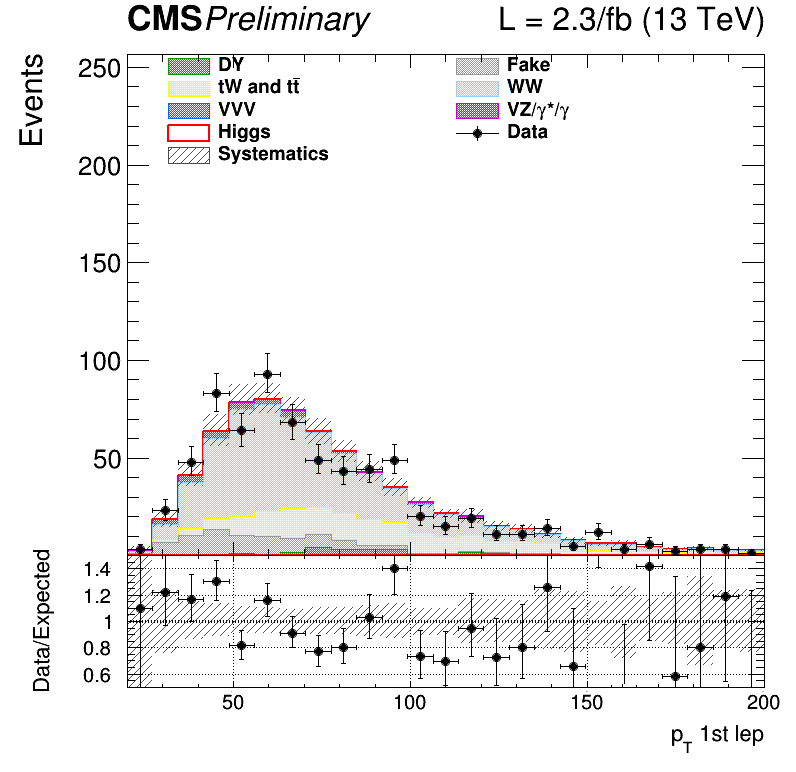
\includegraphics[width=0.45\textwidth]{images/13TeV/cratio_ww2l2v_13TeV_ww_of0j_pt1}
}
\subfigure[0 jets - $\eta^{\ell,1}$]{
  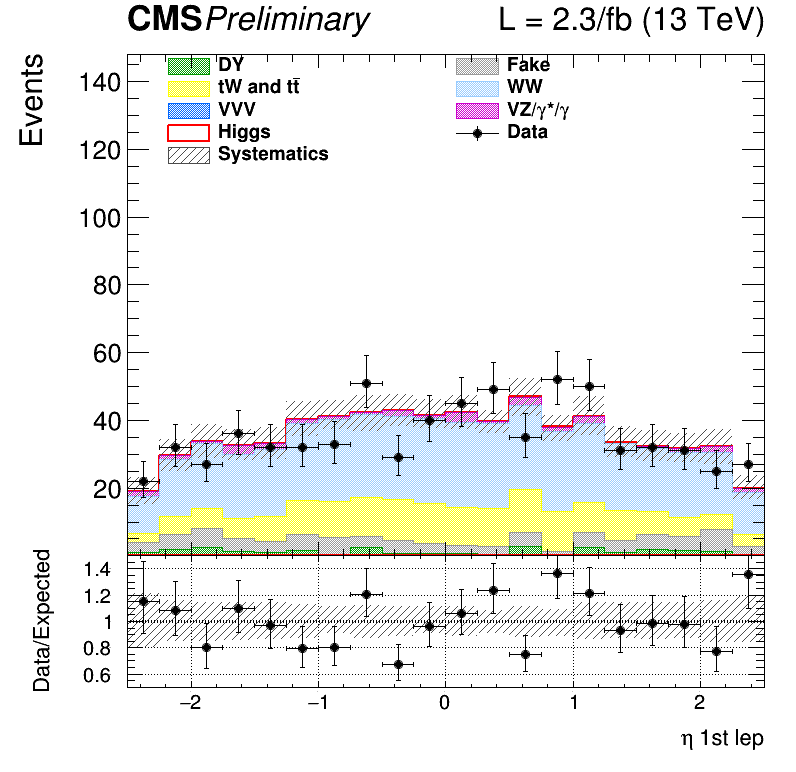
\includegraphics[width=0.45\textwidth]{images/13TeV/cratio_ww2l2v_13TeV_ww_of0j_eta1}
}\\
\subfigure[1 jet - $\pt^{\ell,1}$]{
  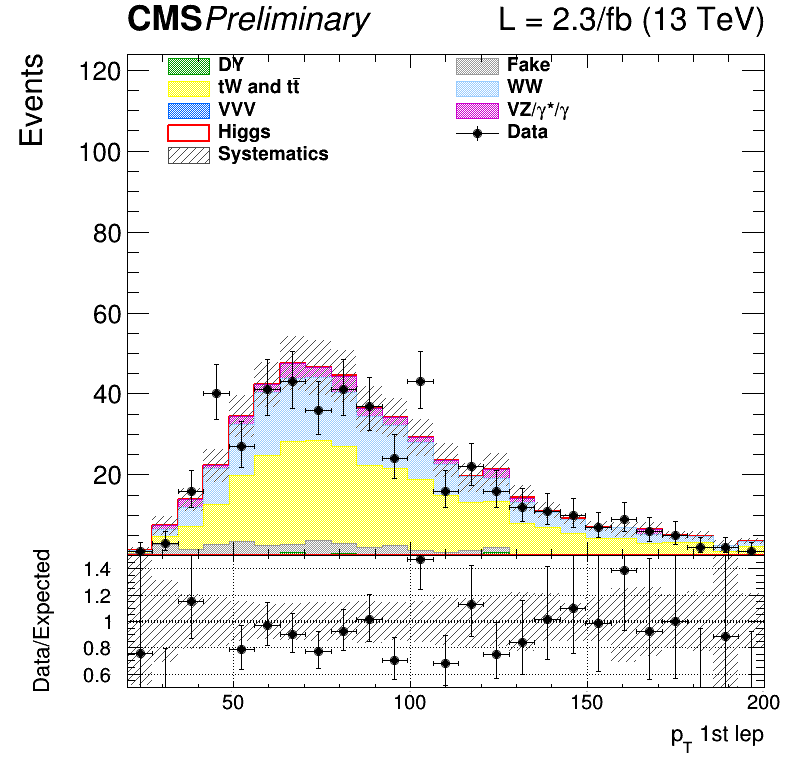
\includegraphics[width=0.45\textwidth]{images/13TeV/cratio_ww2l2v_13TeV_ww_of1j_pt1}
}
\subfigure[1 jet - $\eta^{\ell,1}$]{
  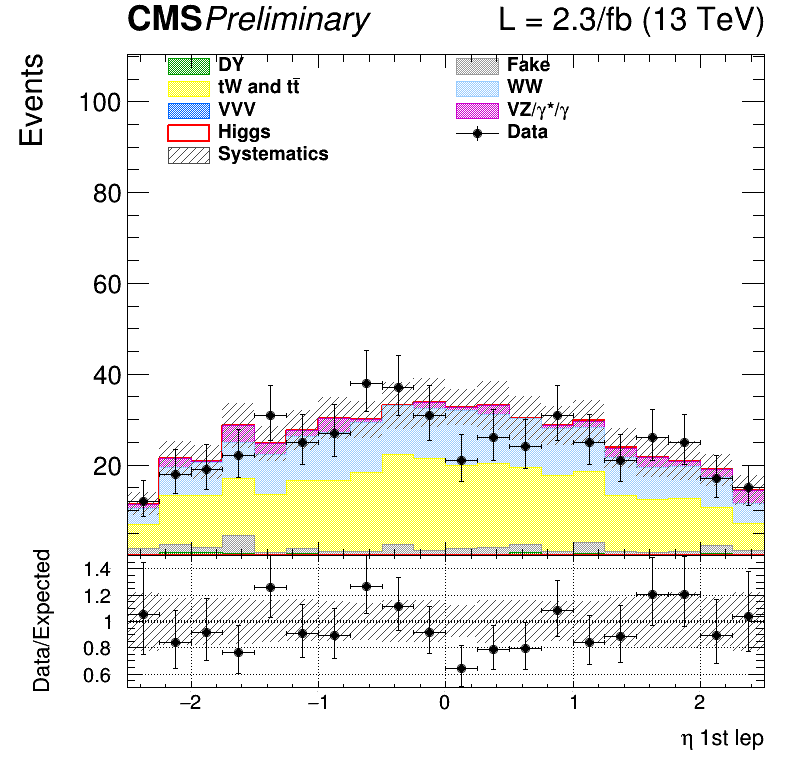
\includegraphics[width=0.45\textwidth]{images/13TeV/cratio_ww2l2v_13TeV_ww_of1j_eta1}
}
\caption{Distributions of \pt (left) and $\eta$ (right) of the leading lepton in events with 0 jets (upper row) and 1 jet (bottom row), for the main backgrounds (stacked histograms), and for a SM Higgs boson signal with $m_\mathrm{H}=125$\GeV (superimposed and stacked red histogram)  after the analysis event selection.}\label{fig:distr1}
\end{figure}

\begin{figure}
\centering
\subfigure[0 jets - $\pt^{\ell,2}$]{
  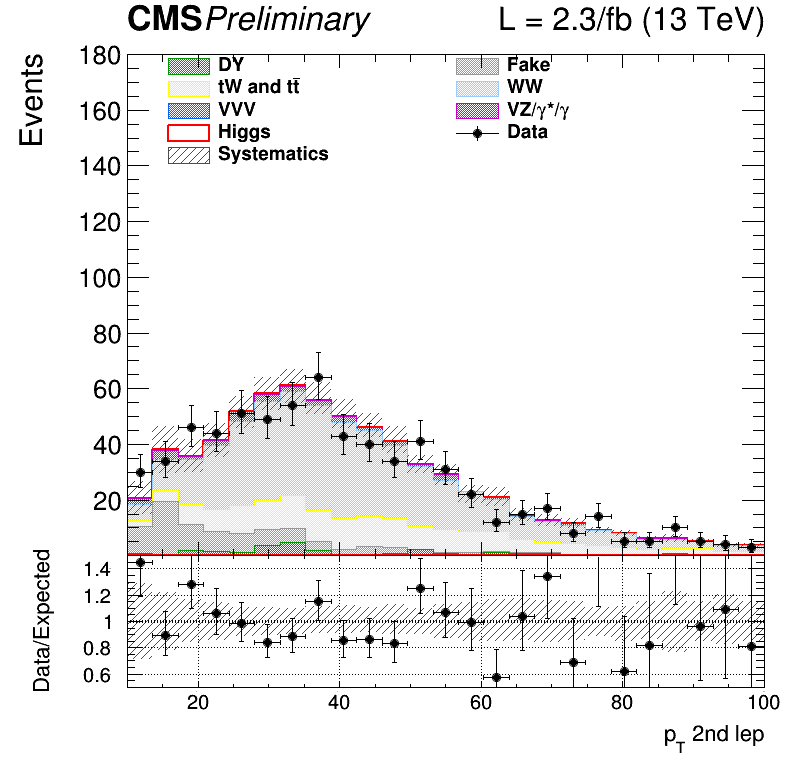
\includegraphics[width=0.45\textwidth]{images/13TeV/cratio_ww2l2v_13TeV_ww_of0j_pt2}
}
\subfigure[0 jets - $\eta^{\ell,2}$]{
  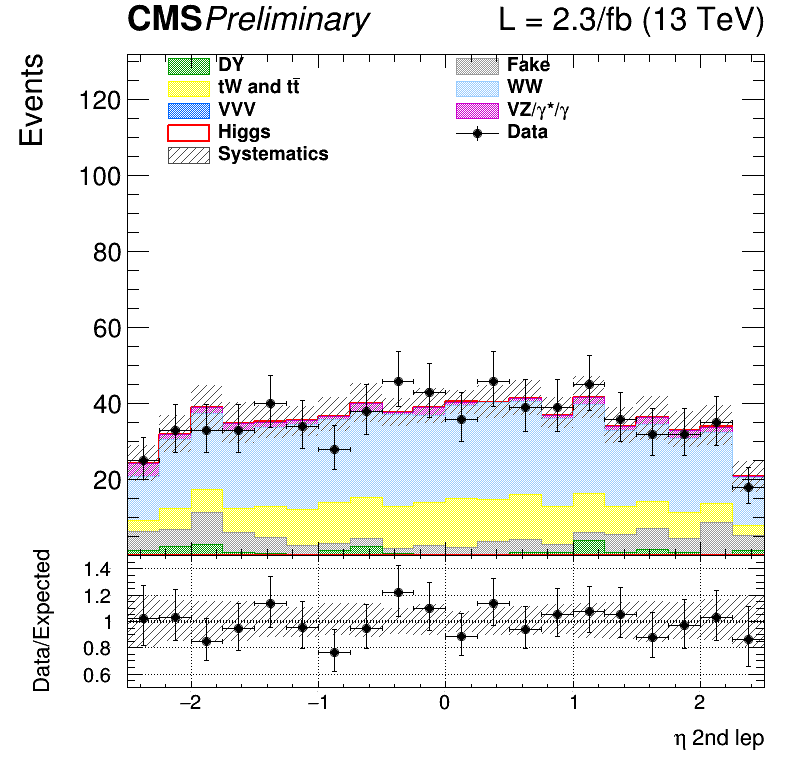
\includegraphics[width=0.45\textwidth]{images/13TeV/cratio_ww2l2v_13TeV_ww_of0j_eta2}
}\\
\subfigure[1 jet - $\pt^{\ell,2}$]{
  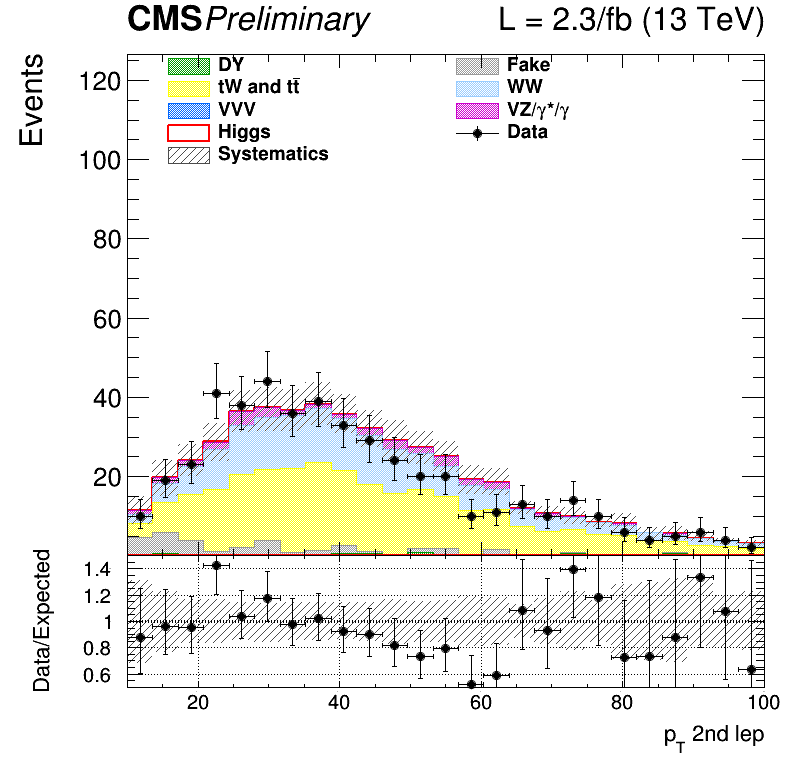
\includegraphics[width=0.45\textwidth]{images/13TeV/cratio_ww2l2v_13TeV_ww_of1j_pt2}
}
\subfigure[1 jet - $\eta^{\ell,2}$]{
  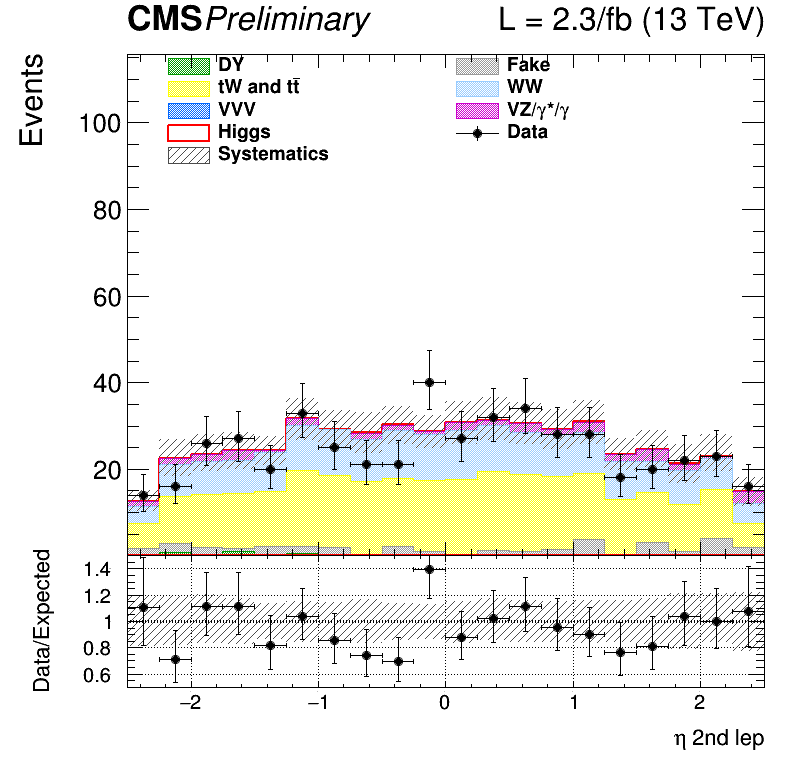
\includegraphics[width=0.45\textwidth]{images/13TeV/cratio_ww2l2v_13TeV_ww_of1j_eta2}
}
\caption{Distributions of \pt (left) and $\eta$ (right) of the subleading lepton in events with 0 jets (upper row) and 1 jet (bottom row), for the main backgrounds (stacked histograms), and for a SM Higgs boson signal with $m_\mathrm{H}=125$\GeV (superimposed and stacked red histogram)  after the analysis event selection.}\label{fig:distr2}
\end{figure}

\begin{figure}
\centering
\subfigure[0 jets - \MET]{
  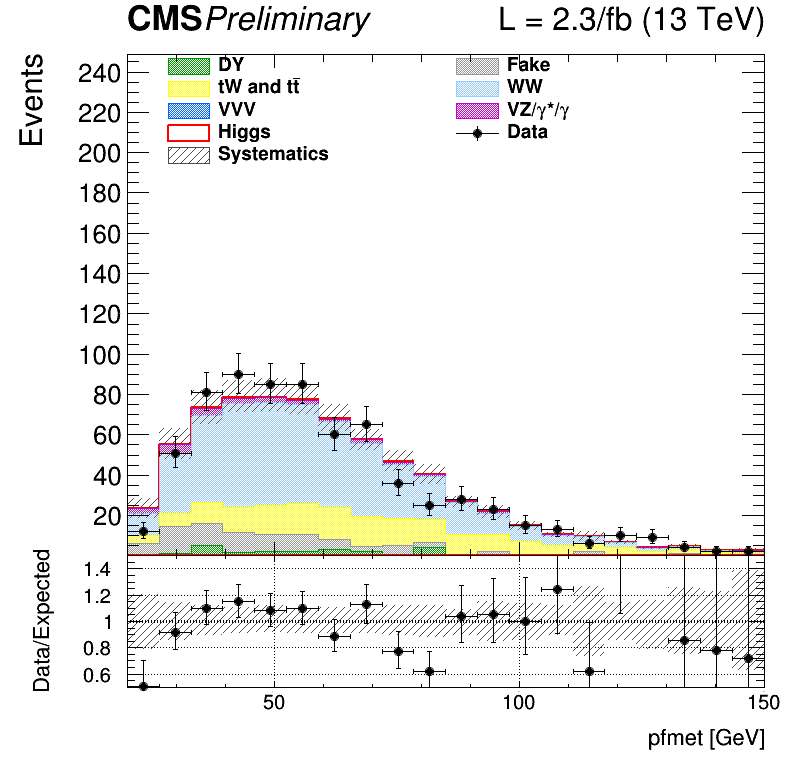
\includegraphics[width=0.45\textwidth]{images/13TeV/cratio_ww2l2v_13TeV_ww_of0j_met}
}
\subfigure[0 jets - \ptll]{
  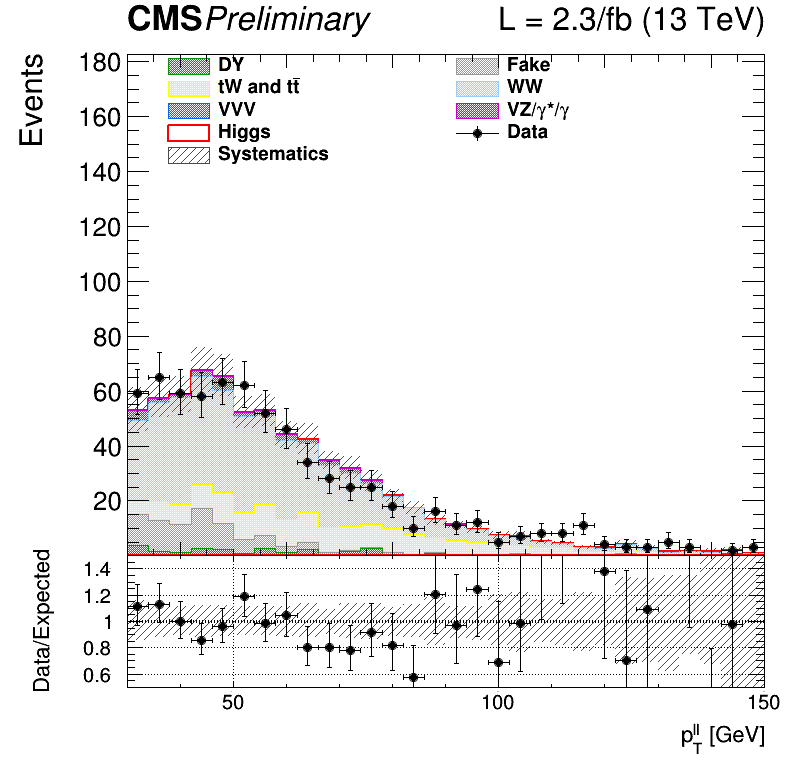
\includegraphics[width=0.45\textwidth]{images/13TeV/cratio_ww2l2v_13TeV_ww_of0j_ptll}
}\\
\subfigure[1 jet - \MET]{
  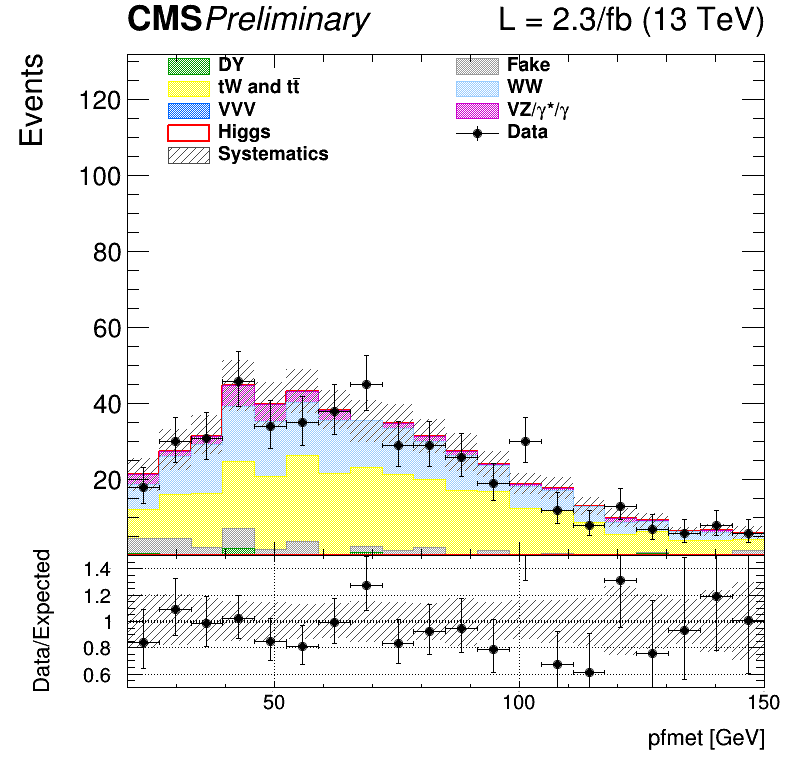
\includegraphics[width=0.45\textwidth]{images/13TeV/cratio_ww2l2v_13TeV_ww_of1j_met}
}
\subfigure[1 jet - \ptll]{
  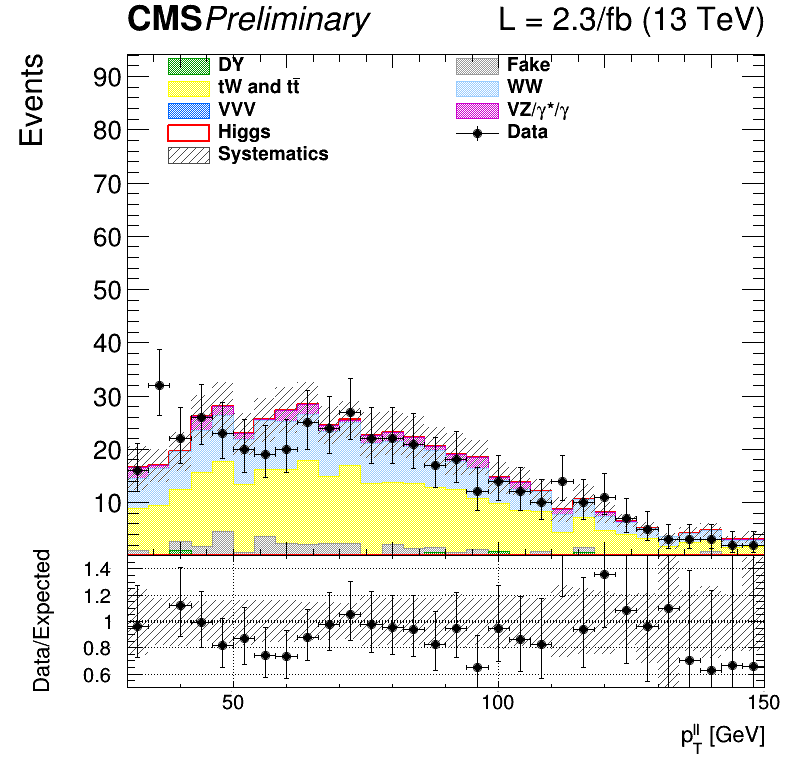
\includegraphics[width=0.45\textwidth]{images/13TeV/cratio_ww2l2v_13TeV_ww_of1j_ptll}
}
\caption{Distributions of \MET (left) and \ptll (right) in events with 0 jets (upper row) and 1 jet (bottom row), for the main backgrounds (stacked histograms), and for a SM Higgs boson signal with $m_\mathrm{H}=125$\GeV (superimposed and stacked red histogram) after the analysis event selection.}\label{fig:distr3}
\end{figure}

An additional categorization is applied in order to increase the signal sensitivity. The 0 ad 1 jets categories are further split according to the lepton flavour to e$\mu$ and $\mu$e, where the first lepton refers to the leading one. In this way an improvement of about 10\% in terms of signal significance can be achieved, exploiting the different W+jets background contribution in the two categories. Actually, this background is characterized by the presence of one jet misidentified as a lepton, and the probability for a jet to be misidentified as a muon is larger than as an electron.

\subsection{Signal extraction}

To extract the Higgs boson signal contribution in the four previously mentioned categories, a similar approach to the one used in the Run 1 analysis~\cite{Chatrchyan:2013iaa} is pursued. The analysis is based on two-dimensional templates of \mll versus \mt to discriminate signal and background contributions. The \mll template is defined using 5 bins from $\mll=10$\GeV up to $\mll=110$\GeV, while for the \mt template 7 bins are defined in the range $60\GeV < \mt < 200$\GeV. The phase space with $\mt<60$\GeV is used as an orthogonal control region to extract the normalization of the \dytt background. A binned maximum likelihood fit to the signal and background two-dimensional templates is performed to extract the signal strength in the four categories.

The statistical methodology used to interpret the data and combine the results from the independent 0 and 1 jets categories in the e$\mu$ and $\mu$e final states has been developed by the ATLAS and CMS collaborations in the context of the LHC Higgs Combination Group~\cite{CMS-NOTE-2011-005,Khachatryan:2014jba}.
The number of events in each category and in each bin of the two-dimensional template is modelled as a Poisson random variable, with a mean value given by the sum of the contributions from all the processes under consideration. Systematic uncertainties are represented by individual nuisance parameters with log-normal distributions. The uncertainties affect the overall normalization of signal and backgrounds, as well as their (\mll, \mt) shape. Correlations between systematic uncertainties in different categories are taken into account. 












